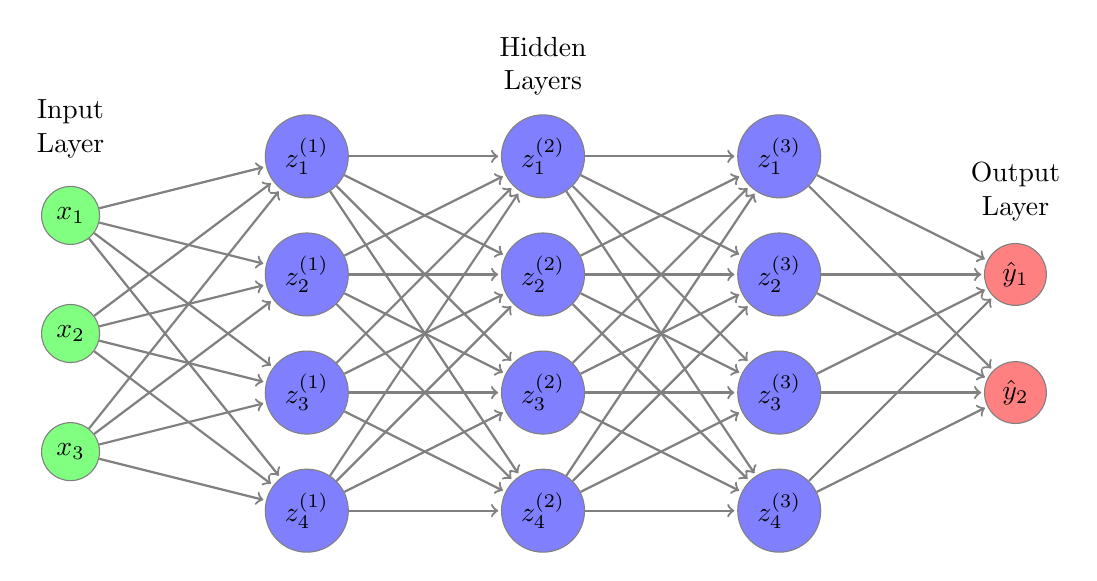
\begin{tikzpicture}[shorten >=1pt, ->, draw=black!50, node distance=1.5cm and 3.5cm, align=center]

    % Styles
    \tikzstyle{input} = [circle, draw, fill=green!50, minimum size=2em]
    \tikzstyle{hidden} = [circle, draw, fill=blue!50, minimum size=2em]
    \tikzstyle{output} = [circle, draw, fill=red!50, minimum size=2em]
    \tikzstyle{connection} = [->, thick]

    % Network Stage Labels
    \node[align=center] at (0,-0.4) {Input \\ Layer};
    \node[align=center] at (6,0.4) {Hidden \\ Layers};
    \node[align=center] at (12,-1.2) {Output \\ Layer};

    % Input Layer
    \foreach \i in {1,2,3}
        \node[input] (I\i) at (0,-\i*1.5) {$x_\i$};

    % Hidden Layer 1
    \foreach \i in {1,2,3,4}
        \node[hidden] (H1\i) at (3,-\i*1.5+0.75) {$z^{(1)}_\i$};

    % Hidden Layer 2
    \foreach \i in {1,2,3,4}
        \node[hidden] (H2\i) at (6,-\i*1.5+0.75) {$z^{(2)}_\i$};

    % Hidden Layer 3
    \foreach \i in {1,2,3,4}
        \node[hidden] (H3\i) at (9,-\i*1.5+0.75) {$z^{(3)}_\i$};

    % Output Layer
    \foreach \i in {1,2}
        \node[output] (O\i) at (12,-\i*1.5-0.75) {$\hat{y}_\i$};

    % Connections from Input to Hidden Layer 1
    \foreach \i in {1,2,3}
        \foreach \j in {1,2,3,4}
            \draw[connection] (I\i) -- (H1\j);

    % Connections from Hidden Layer 1 to Hidden Layer 2
    \foreach \i in {1,2,3,4}
        \foreach \j in {1,2,3,4}
            \draw[connection] (H1\i) -- (H2\j);

    % Connections from Hidden Layer 2 to Hidden Layer 3
    \foreach \i in {1,2,3,4}
        \foreach \j in {1,2,3,4}
            \draw[connection] (H2\i) -- (H3\j);

    % Connections from Hidden Layer 3 to Output Layer
    \foreach \i in {1,2,3,4}
        \foreach \j in {1,2}
            \draw[connection] (H3\i) -- (O\j);

\end{tikzpicture}
